\documentclass{beamer}
%Information to be included in the title page:
\title{Reverse Mode Algorithmic Differentiation}
\author[Group 18]{Callum Firth, Maximilian Fricker, Alexander Le Marchant, Samuel Murdoch}
\institute[Imperial]{Imperial College London}
\date{20th June 2023}
\usetheme{Madrid}

\begin{document}

\frame{\titlepage}

% This may all change but:


% Intro
% Im thinking we start with a brief overview on why care about derivatives and the types of func we are caring about (ie. these are the R^n to R^1 func or similar)
% Then maybe move to the DAG representation of expressions (Talk about how we did this, why dag better)
% 

% RM
% See if we can create a gif? of a traversal of a DAG
% Show both the forward pass to evaluate it and then the backward pass
% Then maybe compare this to the forward mode gif
% Breifly mention complexity of the two algorithms (maybe only care about time here)
% Then talk about difference in time of the two algorithms

% Demo (May swap with conclusion/applications)
% Show basic derivative calculation (think of a nice function so we can easily confirm this)
% Move on to show difference in time between RM and FM (can be for a simple ex of n = 50)
% If completed in time show ODE equation/simulation

% Conclusion/Applications
% Mention theory behind ODE stuff
% Mention theory why we care about the neural network stuff
% Talk about neural networks maybe application on backpropagation, reducing loss func, optimising weights etc

\AtBeginSection[Introduction]
{
\begin{frame}{Outline}
    \tableofcontents[currentsection]
\end{frame}
}

\section{Introduction}

\begin{frame}{Why are Derivatives important?}
\begin{itemize}
    \item Neural Networks
    \begin{itemize}
        \item Loss function / Gradient descent
    \end{itemize}
    \item Systems of non linear equations
\end{itemize}
\end{frame}

\begin{frame}{Types of Differentiation}
\frametitle{Types of differentiation}
Three common ways to differentiate a function on a computer
\begin{itemize}
    \item Finite Differences
    \item Symbolic Differentiation
    \item Algorithmic Differentiation (AD)
\end{itemize}
\end{frame}

\begin{frame}{Function Definition}
    \begin{equation*}
            F: \mathbb{R}^n \longrightarrow \mathbb{R}^m \qquad
            F(x_1, \ldots, x_n) = (y_1, \ldots, y_m)
    \end{equation*}

    \begin{itemize}
        \item We will compare the computational costs of the Jacobian of $F$
    \end{itemize}
    
    \begin{equation*} \label{jacobian}
        F'(x) = \begin{bmatrix}
            \frac{\partial y_1}{\partial x_1} & \cdots & \frac{\partial y_1}{\partial x_n} \\
            \vdots & \ddots & \vdots \\
            \frac{\partial y_m}{\partial x_1} & \cdots & \frac{\partial y_m}{\partial x_n}
        \end{bmatrix} \in \mathbb{R}^{m \times n}
    \end{equation*}
\end{frame}


\begin{frame}{Finite Differences}
    \begin{equation*}
        \frac{\partial F_i (p)}{\partial x_j} \approx \frac{F_i(p+he_j) - F_i(p)}{h}
    \end{equation*}
    \begin{itemize}
        \item Uses a truncated Taylor expansion 
        \item Returns \alert{approximate} value
        \item Low computational costs
        \begin{itemize}
            \item $\mathcal{O}(n) \cdot \text{Cost}(F)$
        \end{itemize}
    \end{itemize}
\end{frame}

\begin{frame}{Symbolic Differentiation}
    \begin{itemize}
        \item Uses computer algebra packages to take derivatives
        \begin{itemize}
            \item Application of chain rule
        \end{itemize}
        \item Calculates derivative at all $x \in \mathbb{R}^n$
        \item Once a solution is found any value can be plugged in
        \item Returns \alert{exact} value up to machine precision
        \item Very high computational cost
        \begin{itemize}
            \item $\mathcal{O}(nm) \cdot \text{Cost}(F)$
        \end{itemize}
    \end{itemize}
\end{frame}

\begin{frame}{Algorithmic Differentiation}
    \begin{itemize}
        \item Two types
            \begin{itemize}
                \item Forward mode
                \item Reverse mode - we will focus on reverse mode
            \end{itemize}
        \item Application of chain rule
        \item Calculates derivative at specified $x \in \mathbb{R}^n$
        \item Returns \alert{exact} value up to machine precision
        \item Low computational costs
            \begin{itemize}
                \item $\mathcal{O}(n) \cdot \text{Cost}(F)$ with forward mode
                \item $\mathcal{O}(m) \cdot \text{Cost}(F)$ with reverse mode
            \end{itemize}
        \item<2-> Blah Blah
    \end{itemize}
\end{frame}


\begin{frame}{Representing expressions}
    \frametitle{How we can represent expressions}
    \begin{equation*} \label{example1}
        F \begin{pmatrix}
            x \\ y \\ z
        \end{pmatrix} = \begin{pmatrix}
            \sin (x^2 y) + e^{x^2} \\ e^{x^2} \log z
        \end{pmatrix}
    \end{equation*}
    \begin{figure}
        \centering
        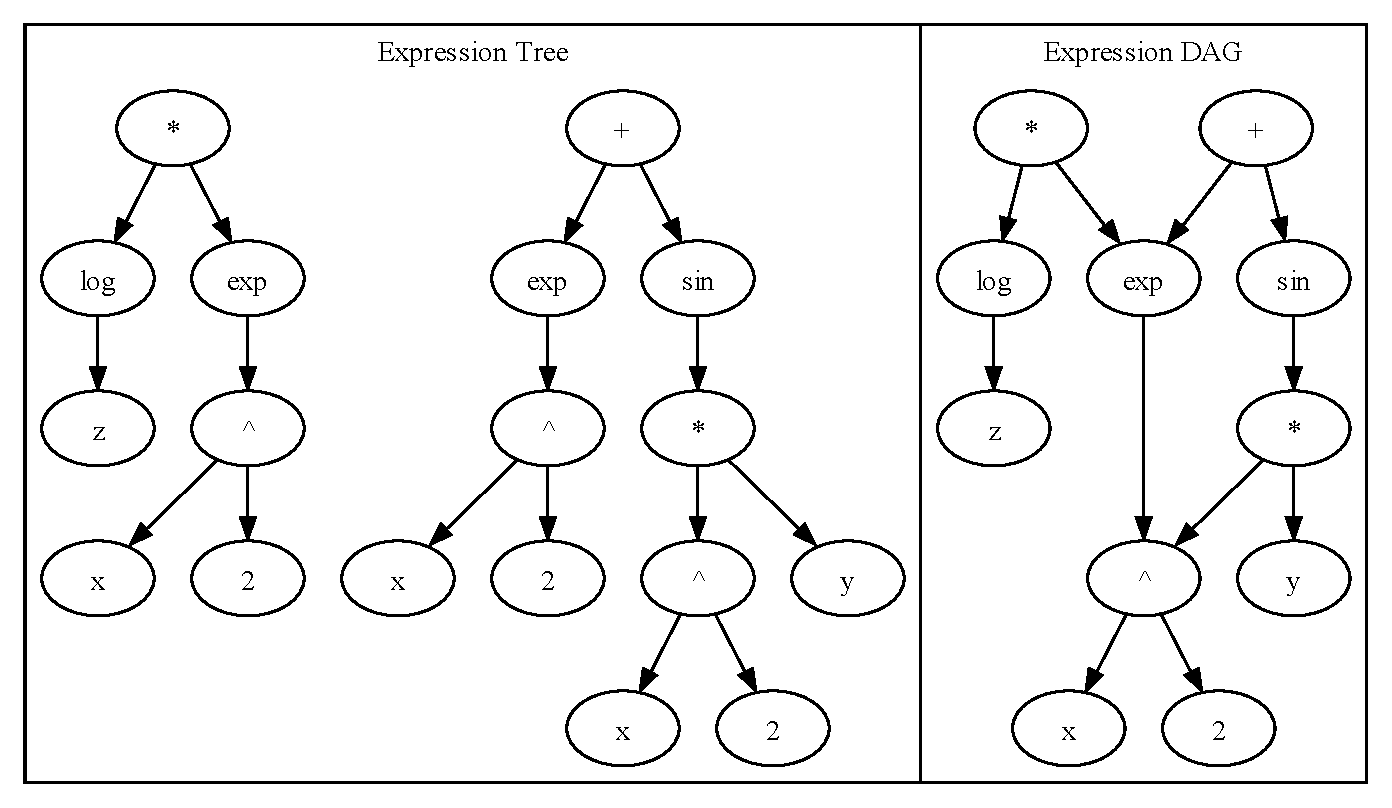
\includegraphics[width=10cm]{images/Graph_Cluster_1.pdf}
        \caption{}
        \label{fig:clusterdag}
    \end{figure}
\end{frame}


\AtBeginSection[Reverse Mode Algorithmic Differentiation]
{
\begin{frame}{Outline}
    \tableofcontents[currentsection]
\end{frame}
}

\section{Reverse Mode Algorithmic Differentiation}

\begin{frame}{Reverse Mode AD}
    \begin{equation*} \label{1df}
            f: \mathbb{R} \longrightarrow \mathbb{R} \qquad
            f(x) = (y)
    \end{equation*}
    \begin{figure}
        \centering
        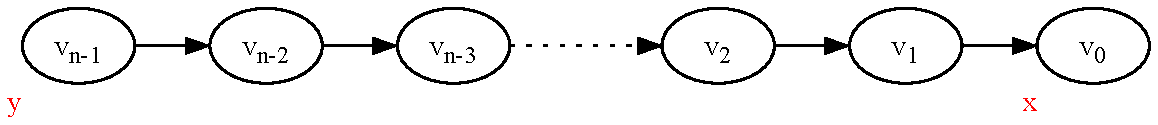
\includegraphics[width=10cm]{images/Graph_simple_expr.pdf}
    \end{figure}
    Applying chain rule
    \begin{equation*}
        \begin{split}
            \frac{\partial y}{\partial x} 
            & = \frac{\partial y}{\partial v_{1}} \frac{\partial v_{1}}{\partial x} \\
            \onslide<2->{& = \left( \frac{\partial y}{\partial v_{2}} \frac{\partial v_{2}}{\partial v_{1}} \right) \frac{\partial v_{1}}{\partial x}} \\
            \onslide<3->{& = \cdots \\
            & = \left( \left( \left( \frac{\partial y}{\partial v_{n-1}} \frac{\partial v_{n-1}}{\partial v_{n-2}} \right) \cdots \right) \frac{\partial v_2}{\partial v_1} \right) \frac{\partial v_1}{\partial x}}
        \end{split}
    \end{equation*}
\end{frame}

\begin{frame}{Reverse Mode AD}
    \begin{itemize}
        \item Quantity of importance is the \alert{adjoint} $\Bar{v}_i$
            \begin{equation*}
                \Bar{v}_i = \frac{\partial y}{\partial v_i}
            \end{equation*}
        \item<2-> Traverse graph forwards computing node values
        \item<3-> Traverse graph backwards computing adjoints
        \item<4-> Rearrange $\Bar{v}_i$ with chain rule
            \begin{equation*}
                \Bar{v}_i = \frac{\partial y}{\partial v_{i+1}} \frac{\partial v_{i+1}}{\partial v_i} = \Bar{v}_{i+1} \frac{\partial v_{i+1}}{\partial v_i}
            \end{equation*}
        \item<5-> Calculate $\Bar{v}_i$ using stored values from forward pass
    \end{itemize}
\end{frame}

\begin{frame}{Adjoint}
    \begin{figure}
        \centering
        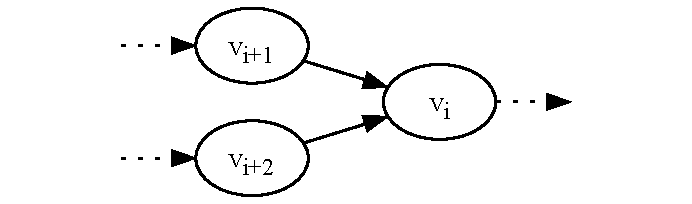
\includegraphics[width=6cm]{images/Graph_simple_parent.pdf}
    \end{figure}
    If $\Bar{v}_1$ has two parents then
    \begin{equation*}
        \Bar{v}_i = \Bar{v}_{i+1} \frac{\partial v_{i+1}}{\partial v_i} + \Bar{v}_{i+2} \frac{\partial v_{i+2}}{\partial v_i}
    \end{equation*}
    \onslide<2->{In general form
    \begin{equation*}
        \Bar{v}_i = \sum_{j \in \{\text{parents of } i\}} \Bar{v}_j \frac{\partial v_j}{\partial v_i}
    \end{equation*}
    }
\end{frame}


\AtBeginSection[Example]{\begin{frame}{Outline}
    \tableofcontents[currentsection]
\end{frame}}
\section{Example}

\begin{frame}{Forward Pass}
\frametitle{Forward Pass}
Function: $F(x, y) = \sin(x^2 y) + \exp(x^2)$

Conditions: ${x:1, y:2}$
\begin{figure}[h!]
    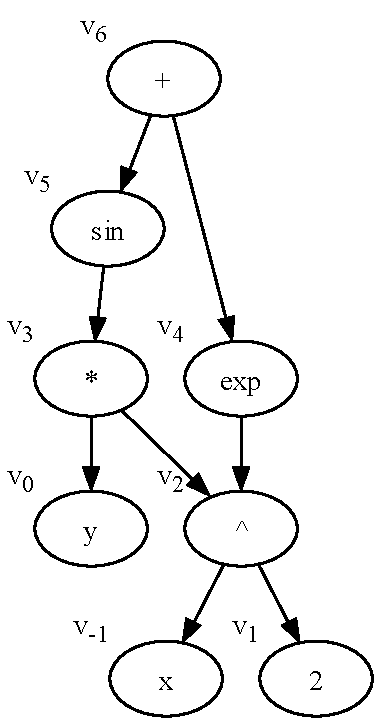
\includegraphics[width=3cm]{images/Graph_simple_example.pdf}
    \label{fig:DAGgraph}
\end{figure}

\end{frame}

\begin{frame}{Forward Pass}

Function: $F(x, y) = \sin(x^2 y) + \exp(x^2)$

Conditions: ${x:1, y:2}$
\begin{center}
        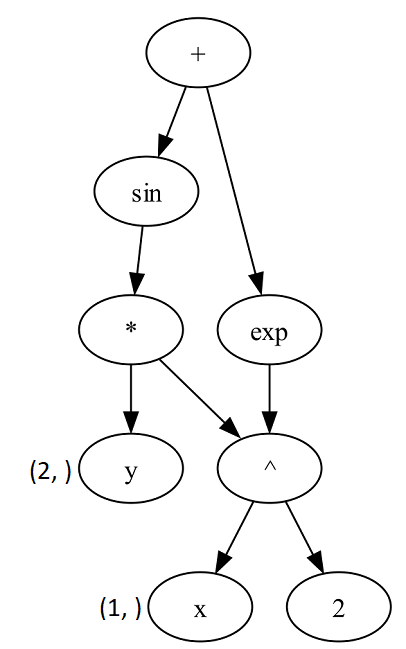
\includegraphics[width=4cm]{DAG_gif_images/fwd_1_fix_1.png}
\end{center}
\end{frame}

\begin{frame}{Forward Pass}

Function: $F(x, y) = \sin(x^2 y) + \exp(x^2)$

Conditions: ${x:1, y:2}$
\begin{center}
        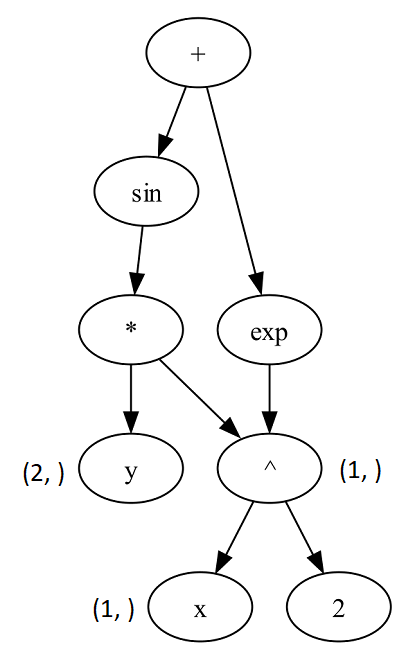
\includegraphics[width=4cm]{DAG_gif_images/fwd_1_fix_2.png}
\end{center}
\end{frame}

\begin{frame}{Forward Pass}

Function: $F(x, y) = \sin(x^2 y) + \exp(x^2)$

Conditions: ${x:1, y:2}$
\begin{center}
        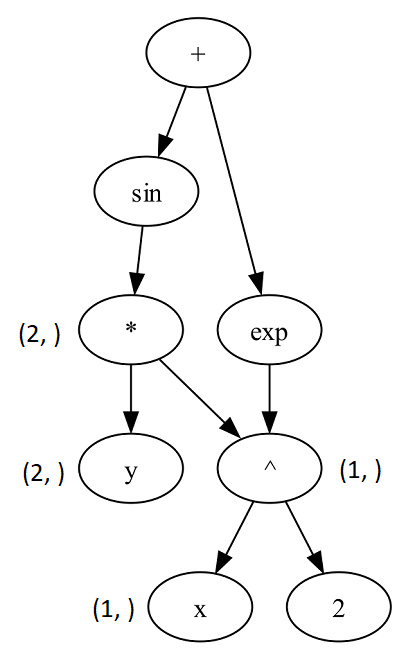
\includegraphics[width=4cm]{DAG_gif_images/fwd_1_fix_3.png}
\end{center}
\end{frame}

\begin{frame}{Forward Pass}

Function: $F(x, y) = \sin(x^2 y) + \exp(x^2)$

Conditions: ${x:1, y:2}$
\begin{center}
        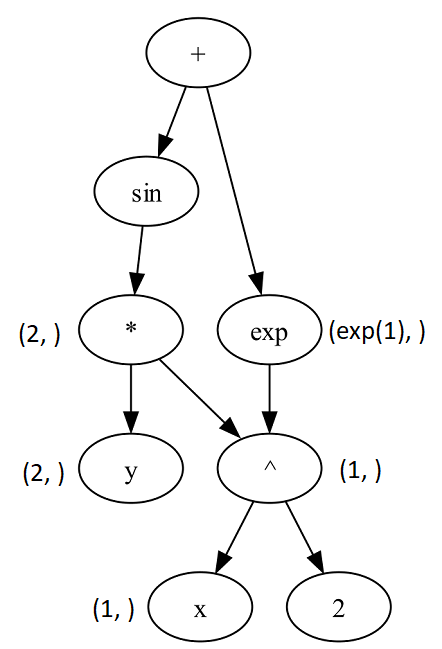
\includegraphics[width=4cm]{DAG_gif_images/fwd_1_fix_4.png}
\end{center}
\end{frame}

\begin{frame}{Forward Pass}

Function: $F(x, y) = \sin(x^2 y) + \exp(x^2)$

Conditions: ${x:1, y:2}$
\begin{center}
        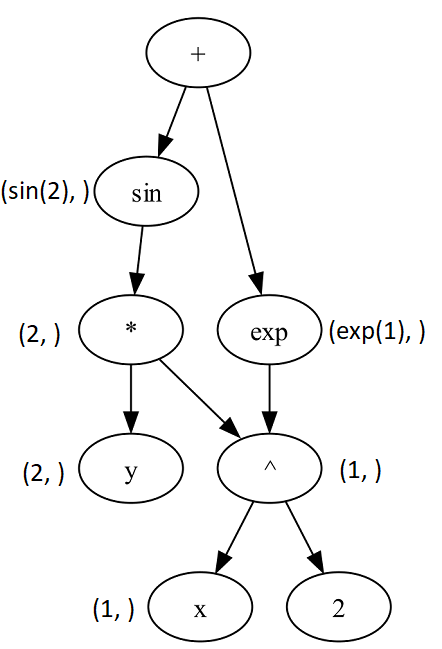
\includegraphics[width=4cm]{DAG_gif_images/fwd_1_fix_5.png}
\end{center}
\end{frame}

\begin{frame}{Forward Pass}

Function: $F(x, y) = \sin(x^2 y) + \exp(x^2)$

Conditions: ${x:1, y:2}$
\begin{center}
        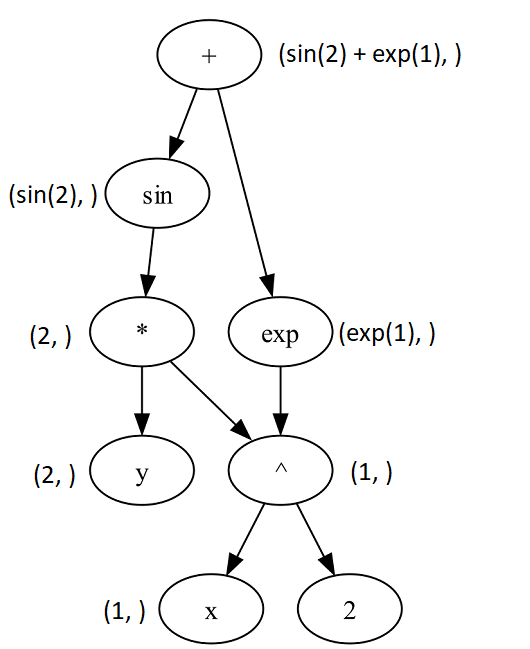
\includegraphics[width=4cm]{DAG_gif_images/fwd_1_fix_6.png}
\end{center}
\end{frame}

\begin{frame}{Reverse Pass}
\frametitle{Reverse Pass}

Function: $F(x, y) = \sin(x^2 y) + \exp(x^2)$

Conditions: ${x:1, y:2}$
\begin{center}
    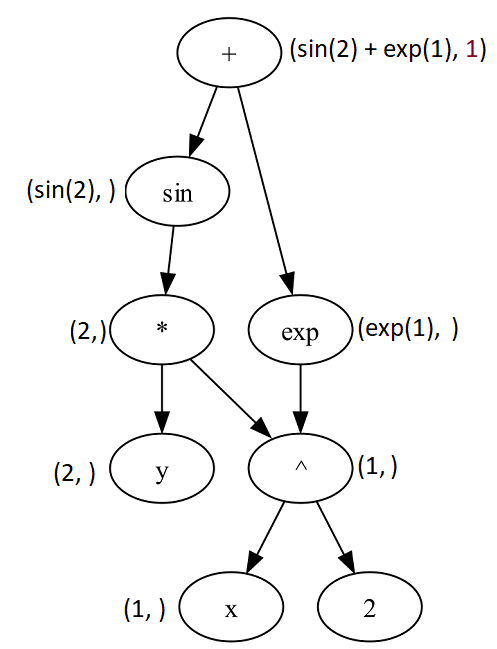
\includegraphics[width=4cm]{DAG_gif_images/rv_1_fix_1.png}
\end{center}
\end{frame}

\begin{frame}{Reverse Pass}
\frametitle{Reverse Pass}

Function: $F(x, y) = \sin(x^2 y) + \exp(x^2)$

Conditions: ${x:1, y:2}$
\begin{center}
    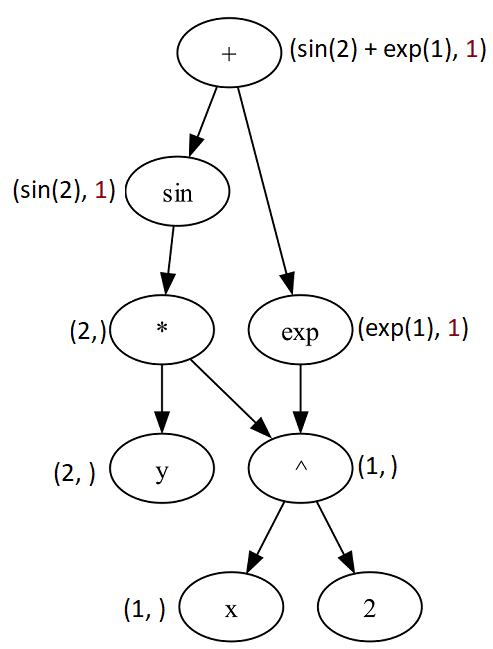
\includegraphics[width=4cm]{DAG_gif_images/rv_1_fix_2.png}
\end{center}
\end{frame}

\begin{frame}{Reverse Pass}
\frametitle{Reverse Pass}

Function: $F(x, y) = \sin(x^2 y) + \exp(x^2)$

Conditions: ${x:1, y:2}$
\begin{center}
    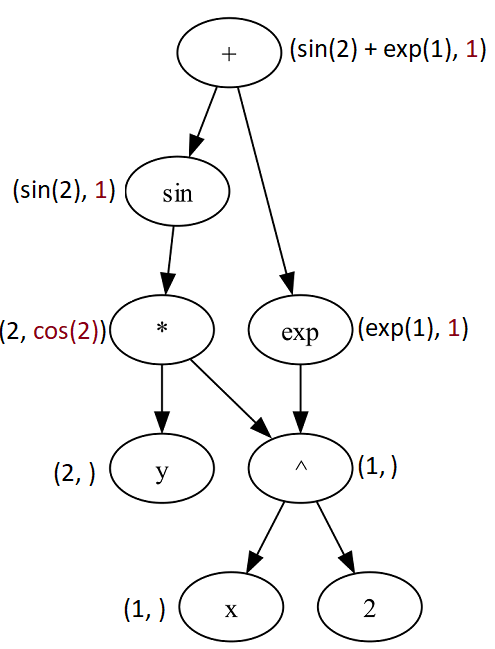
\includegraphics[width=4cm]{DAG_gif_images/rv_1_fix_3.png}
\end{center}
\end{frame}

\begin{frame}{Reverse Pass}
\frametitle{Reverse Pass}

Function: $F(x, y) = \sin(x^2 y) + \exp(x^2)$

Conditions: ${x:1, y:2}$
\begin{center}
    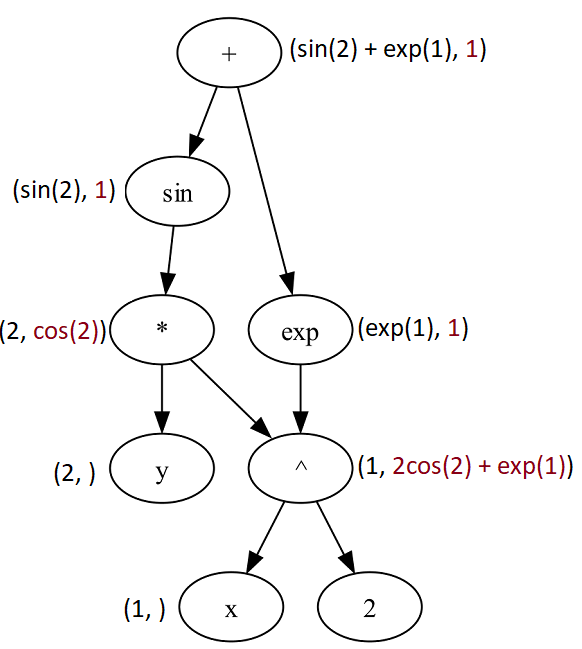
\includegraphics[width=4cm]{DAG_gif_images/rv_1_fix_4.png}
\end{center}
\end{frame}

\begin{frame}{Reverse Pass}
\frametitle{Reverse Pass}

Function: $F(x, y) = \sin(x^2 y) + \exp(x^2)$

Conditions: ${x:1, y:2}$
\begin{center}
    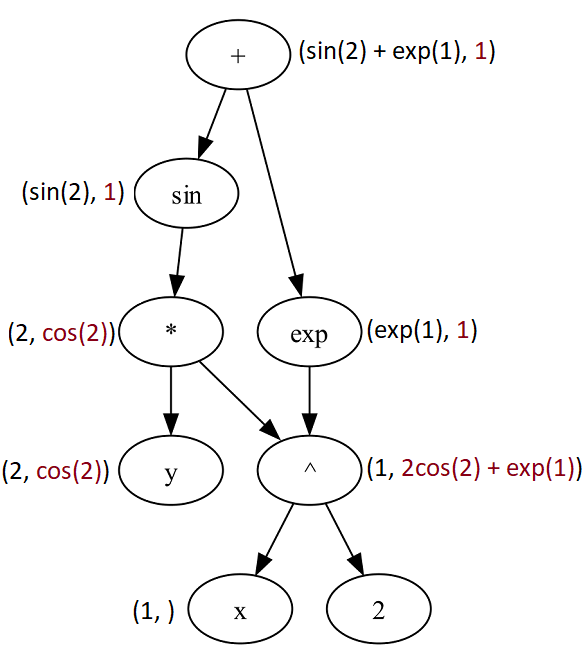
\includegraphics[width=4cm]{DAG_gif_images/rv_1_fix_5.png}
\end{center}
\end{frame}

\begin{frame}{Reverse Pass}
\frametitle{Reverse Pass}

Function: $F(x, y) = \sin(x^2 y) + \exp(x^2)$

Conditions: ${x:1, y:2}$
\begin{center}
    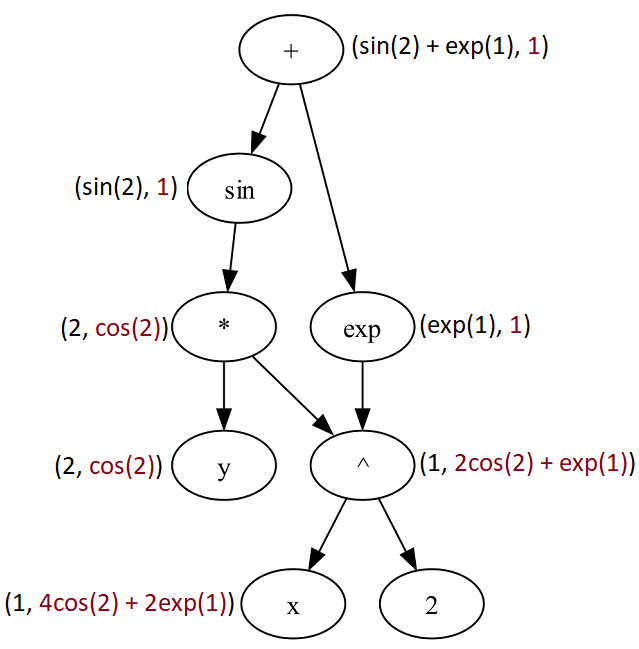
\includegraphics[width=4cm]{DAG_gif_images/rv_1_fix_6.png}
\end{center}
\end{frame}

\begin{frame}{Time Complexity}
\frametitle{Time Efficiency}
For 4 functions $F: \mathbb{R}^n \rightarrow \mathbb{R}$
here are 4 graphs of $n$ against the time taken for both Forward and Backward modes.
\begin{center}
    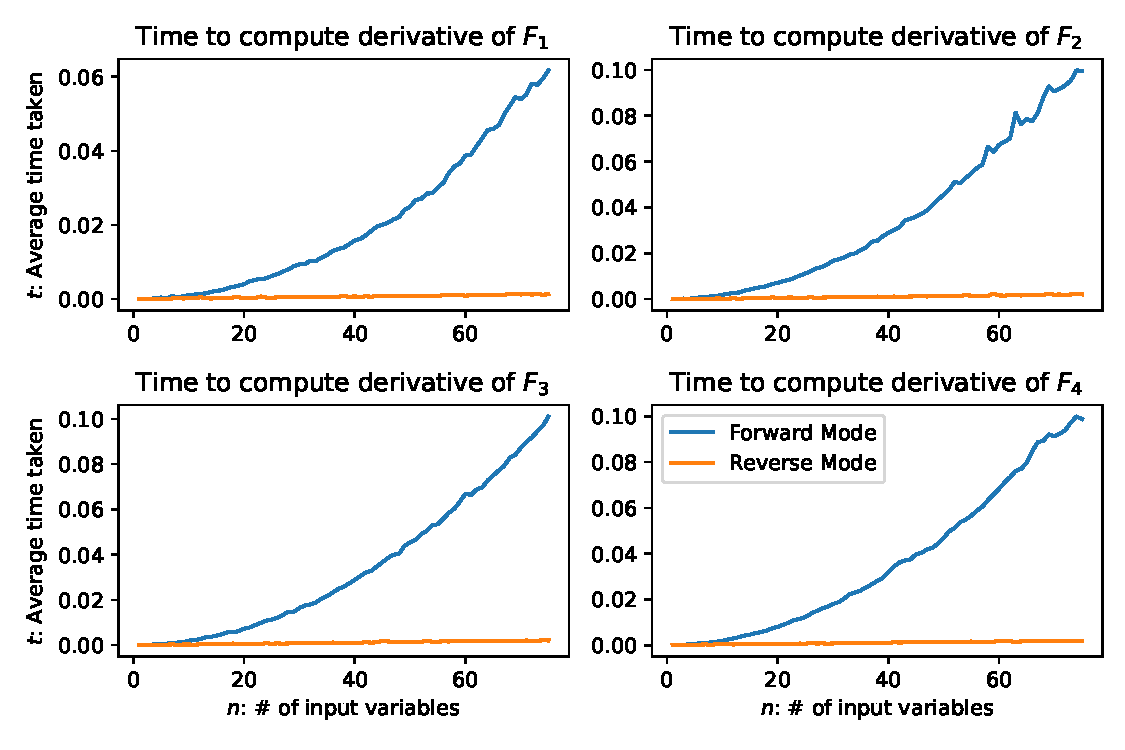
\includegraphics[width=8cm]{images/Graph_TimeDiff.pdf}
\end{center}

As you can see Forward mode (in blue) becomes far less time efficient as n increases, regardless of the function, as predicted.
\end{frame}


\AtBeginSection[Extensions and accuracy]{\begin{frame}{Outline}
    \tableofcontents[currentsection]
\end{frame}}
\section{Extensions and accuracy}


\begin{frame}{Taylor Tests}
\frametitle{Taylor Tests}
Get an estimate for $\mathcal{O}(\epsilon ^ 2)$ by using the equation:
\begin{center}
    $F(x + \epsilon V) = F(x) + \frac{dF}{dx} \cdot \epsilon V + \mathcal{O}(\epsilon ^ 2)$
\end{center}

\begin{center}
    $F(x, y) = x*sin(x+y)$
    
    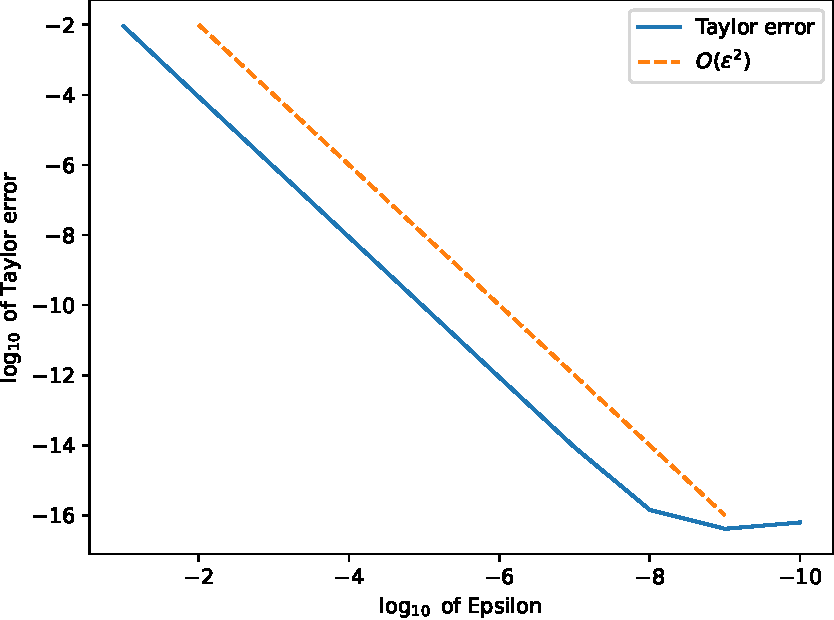
\includegraphics[width=5cm]{images/taylor_error_1.pdf}
\end{center}

Take the gradient using the equation: $\frac{\log{\frac{\|u_1 - u\|}{\|u_2 - u\|}}}{\log{\frac{|h_1|}{|h_2|}}} = \frac{\log\|u_1 - u\| - \log\|u_2 - u\|}{\log|h_1| - \log|h_2|}$
\end{frame}

\begin{frame}
\frametitle{Advection Diffusion Equation}

1 Dimensional Advection Diffusion equation.

\begin{center}
    $\frac{\partial C}{\partial t} = - V\frac{\partial C}{\partial x} + D\frac{\partial^2 C}{\partial x^2}$
\end{center}

Given initial conditions as C as a function of F:

\begin{figure}
\centering
    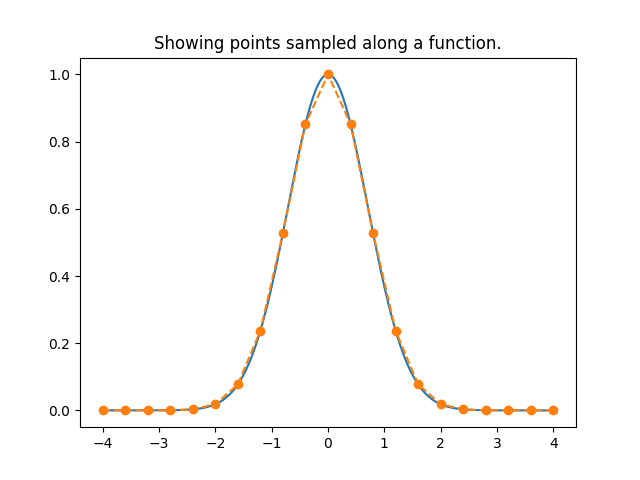
\includegraphics[width=7cm]{images/show_sampling.png}
    \label{fig:sampling}
\end{figure}

\end{frame}

\begin{frame}
\frametitle{More: Advection diffusion equation}

Defining A to be a first-order central differences matrix and B to be a second-order central differences matrix. Then our equation reduces to:
\begin{center}
    $C^{t+1} = C^{t} + \Delta t (-VA + DB) C^{t+1}$
\end{center}

Which rearranges to:

\begin{center}
    $C^{t+1} = M^{-1} C^{t}$
    
    $M := I + \Delta t(VA - DB)$
\end{center}

\end{frame}


\begin{frame}
\frametitle{More: Advection diffusion equation}

\begin{figure}[h]
    \centering
    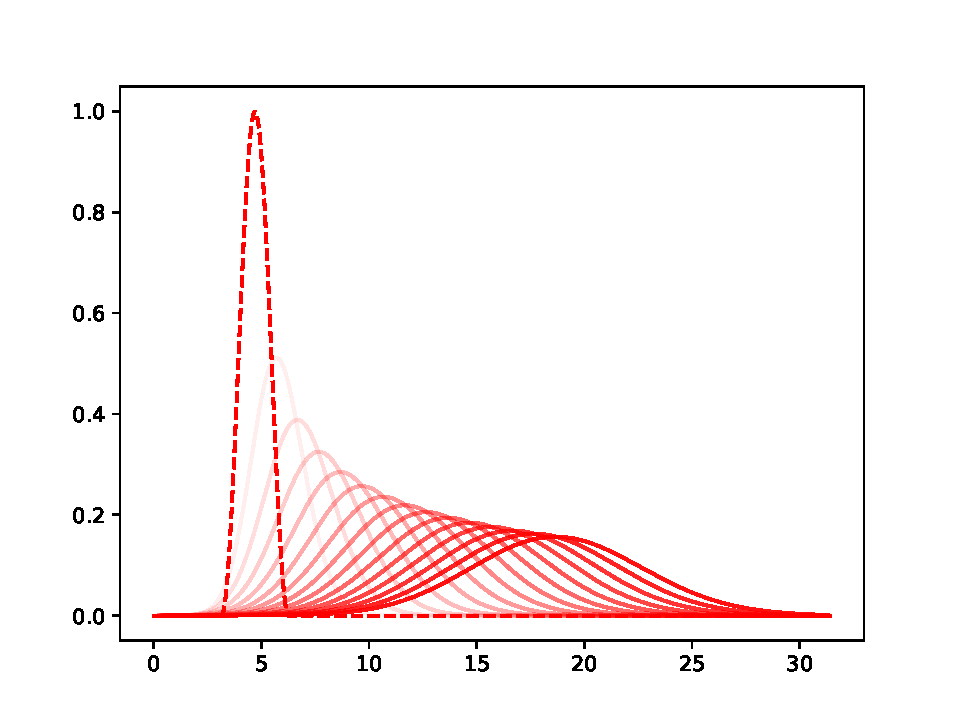
\includegraphics[width=8cm]{images/Figure_1_ODE2.pdf}
    \caption{Plot of ADE with V=10, D=5, plotting from t=0 to t=1.5 at timesteps of 0.1. Dotted line is value at t=0}
    \label{fig:ODE}
\end{figure}

\end{frame}


\begin{frame}
\frametitle{Adjoint of this}

When stepping forward in time we have that:

\begin{center}
    $C^{t+1} = M^{-1} C^{t}$
\end{center}

When working with matrices the adjoint function is always the transpose, so we get that:

\begin{center}
    $\Bar{C}^{t} = M^{-T} \Bar{C}^{t+1}$
\end{center}

\end{frame}

\begin{frame}{Uses of calculating the Adjoint}

When calculating the Adjoint of these we output $\frac{\partial C}{\partial t}$ as an array with the derivative at each $C_i$. These values show us how much of an effect changing each point will have on the final outcome.

\begin{center}
    $[\frac{\partial C_0}{\partial t}, \frac{\partial C_1}{\partial t}, \frac{\partial C_2}{\partial t}, ..., \frac{\partial C_{n-1}}{\partial t}]$
\end{center}


This can be useful for modeling pollution to figure out how increasing pollution in one area will affect the surrounding areas later on.

\end{frame}

\end{document}